% arara: xelatex
% arara: bibtex
% arara: xelatex
% arara: xelatex
% arara: clean: { files: [ main.aux, main.bbl ] }
% arara: clean: { files: [ main.bcf, main.cod ] } 
% arara: clean: { files: [ main.blg, main.lof ] }
% arara: clean: { files: [ main.lot, main.out ] } 
% arara: clean: { files: [ main.toc, main.run.xml ] }
% 
% The document can still be compiled with XeLaTex and BibTeX as usual
%
\documentclass[aspectratio=169,hideallsubsections]{beamer}

\usepackage{polyglossia}
\usepackage{graphicx}
\usepackage{fontspec}
\usepackage{tikz}

\usepackage{qname}


\setprefix{ldn}{http://www.w3.org/ns/ldn\#}
\setprefix{ldp}{http://www.w3.org/ns/ldp\#}

\setmainlanguage{english}

\usetheme{metropolis}
\usefonttheme{opensans}
% \usetheme{Goettingen}
% \usecolortheme{sidebartab}
% blau: 5294e2
% dunkel: 343944

% \definecolor{mDarkBrown}{HTML}{604c38}
\definecolor{mDarkTeal}{HTML}{343944}   % dark color
\definecolor{mLightBrown}{HTML}{5294E2} % highlight
% \definecolor{mLightGreen}{HTML}{14B03D}
% \setbeamertemplate{navigation symbols}{}
\setbeamertemplate{footline}[frame number]

% 15 min



% Set style for listings
\definecolor{backgray}{rgb}{0.9,0.9,0.9}
\setmonofont{DejaVuSansMono}[
    Scale=.8,
    Extension=.ttf,
    UprightFont=*,
    BoldFont=*-Bold
]
% \newfontfamily{\lstfamily}[Scale=.697]{DejaVuSansMono.ttf}
% \newfontfamily{\lstfamily}[Scale=.697]{\ttfamily}
\lstset{
        breaklines=true,
        basicstyle=\ttfamily,
        breakindent=1em,
%         prebreak={\mbox{\,$\neg$}},
        prebreak={\mbox{\,↵}},
        captionpos=b,
        escapeinside={/*@}{@*/},
        float=tbhp,
        showstringspaces=false,
        backgroundcolor=\color{backgray},
        linewidth=\columnwidth,
        xleftmargin=.5em,
        xrightmargin=0pt,
        framexleftmargin=.5em,
        framexrightmargin=0pt
}

\usepackage{graphicx}
\usepackage{listings}
\setcounter{tocdepth}{1}

\title{Linked Data Notifications}
\subtitle{Distributed Update Notification and Propagation on the Web of Data}
\author{Natanael Arndt}
\date{August 29, 2016 (modified September 2, 2016)}
\institute{AKSW Colloquium}

\begin{document}
% Title
\metroset{background=dark}
\maketitle
\metroset{background=light}

\section{Motivation and Problem}
\begin{frame}
  \frametitle{\insertsection}%

\tikz[remember picture,overlay] \node[inner sep=0pt,anchor=east,transform canvas={yshift = -.5cm}] at (current page.east){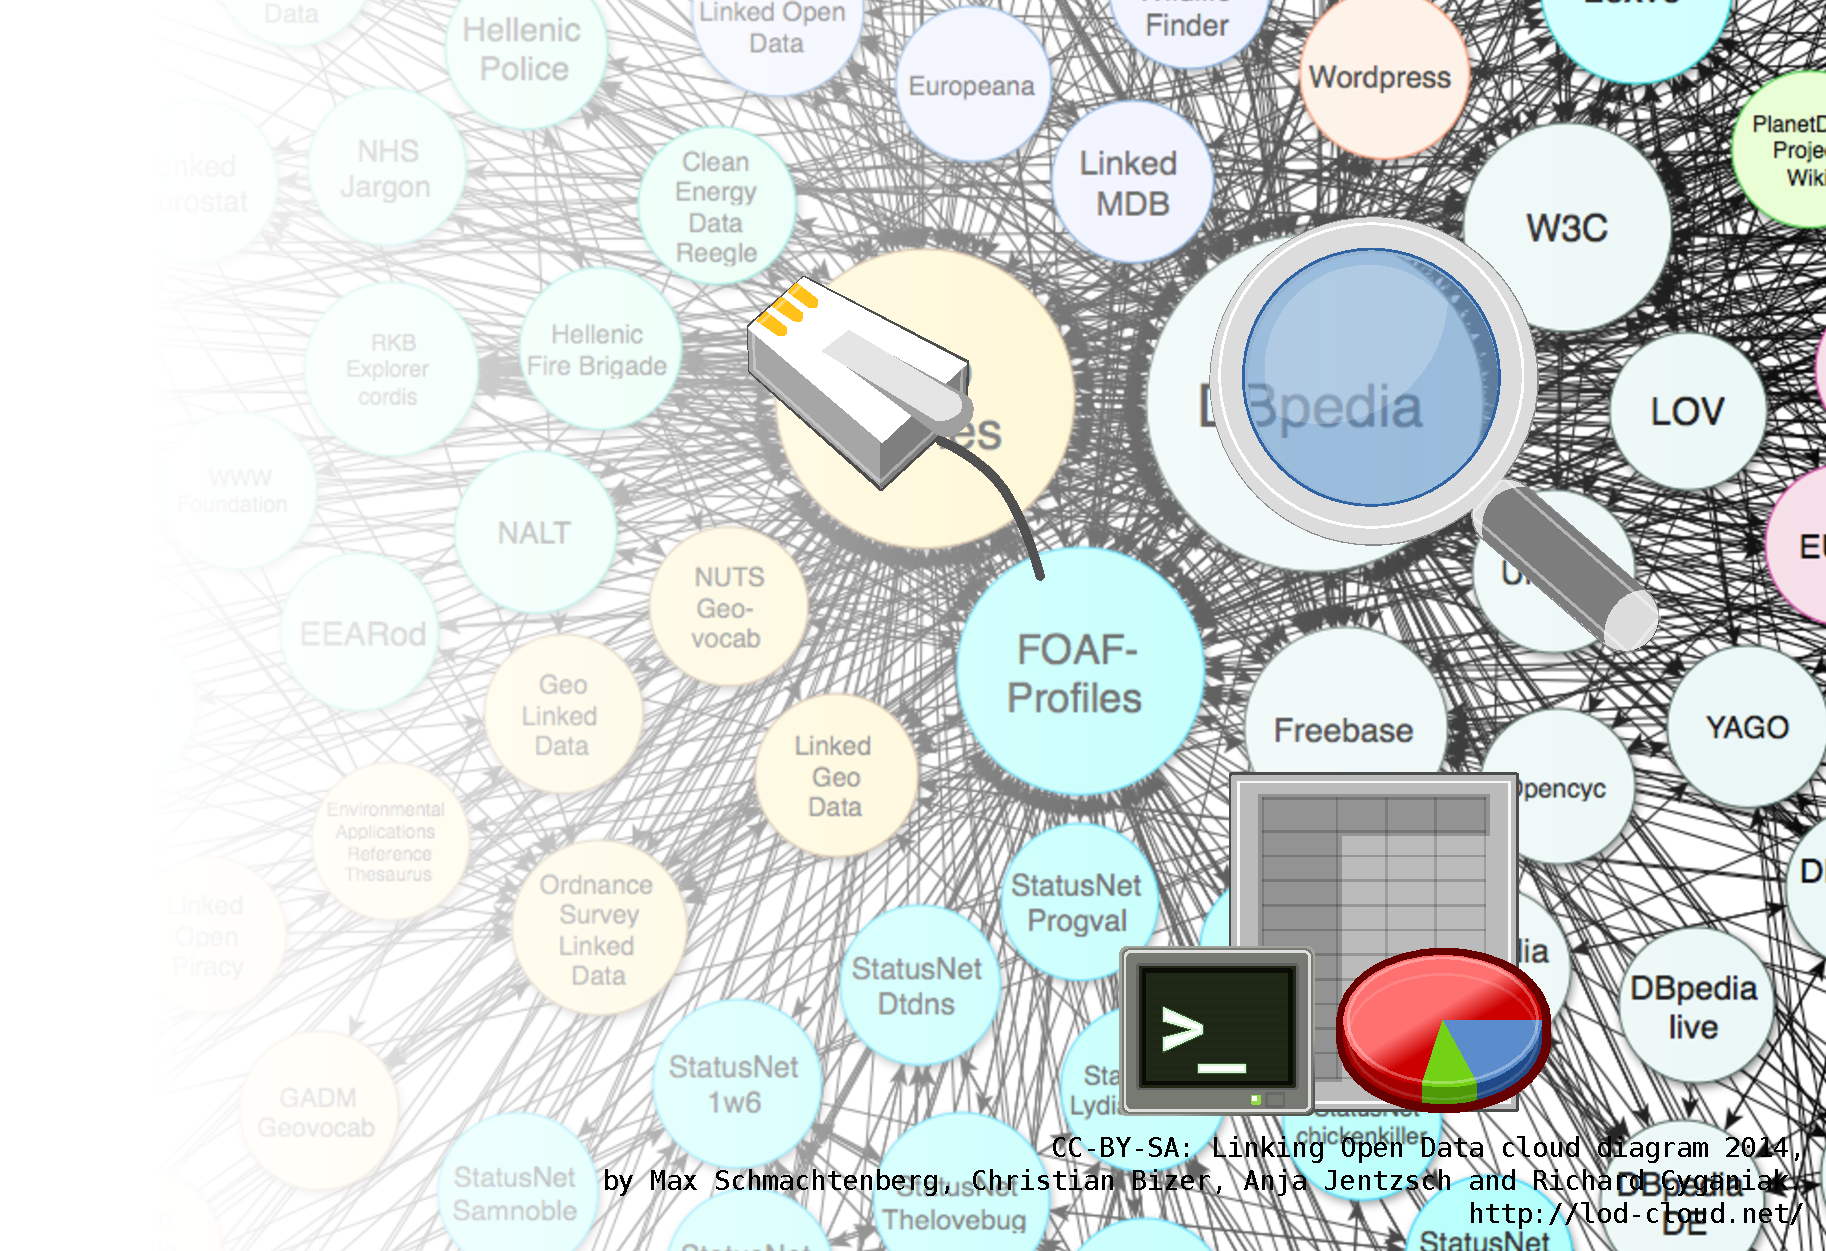
\includegraphics[width=.5\textwidth]{LOD-Cloud-2014}};
\begin{minipage}{\textwidth}
  \begin{itemize}
  \item The Web of Data is a highly interlinked Data Cloud
  \item This enables us to …
  \begin{itemize}
  \item retrieve structured data about things
  \item discover links among datasets
  \item answer questions involving multiple datasets
  \end{itemize}
  \end{itemize}
\end{minipage}%
\end{frame}


\begin{frame}
  \frametitle{\insertsection}%
  
\tikz[remember picture,overlay] \node[inner sep=0pt,anchor=east,transform canvas={yshift = -.5cm}] at (current page.east){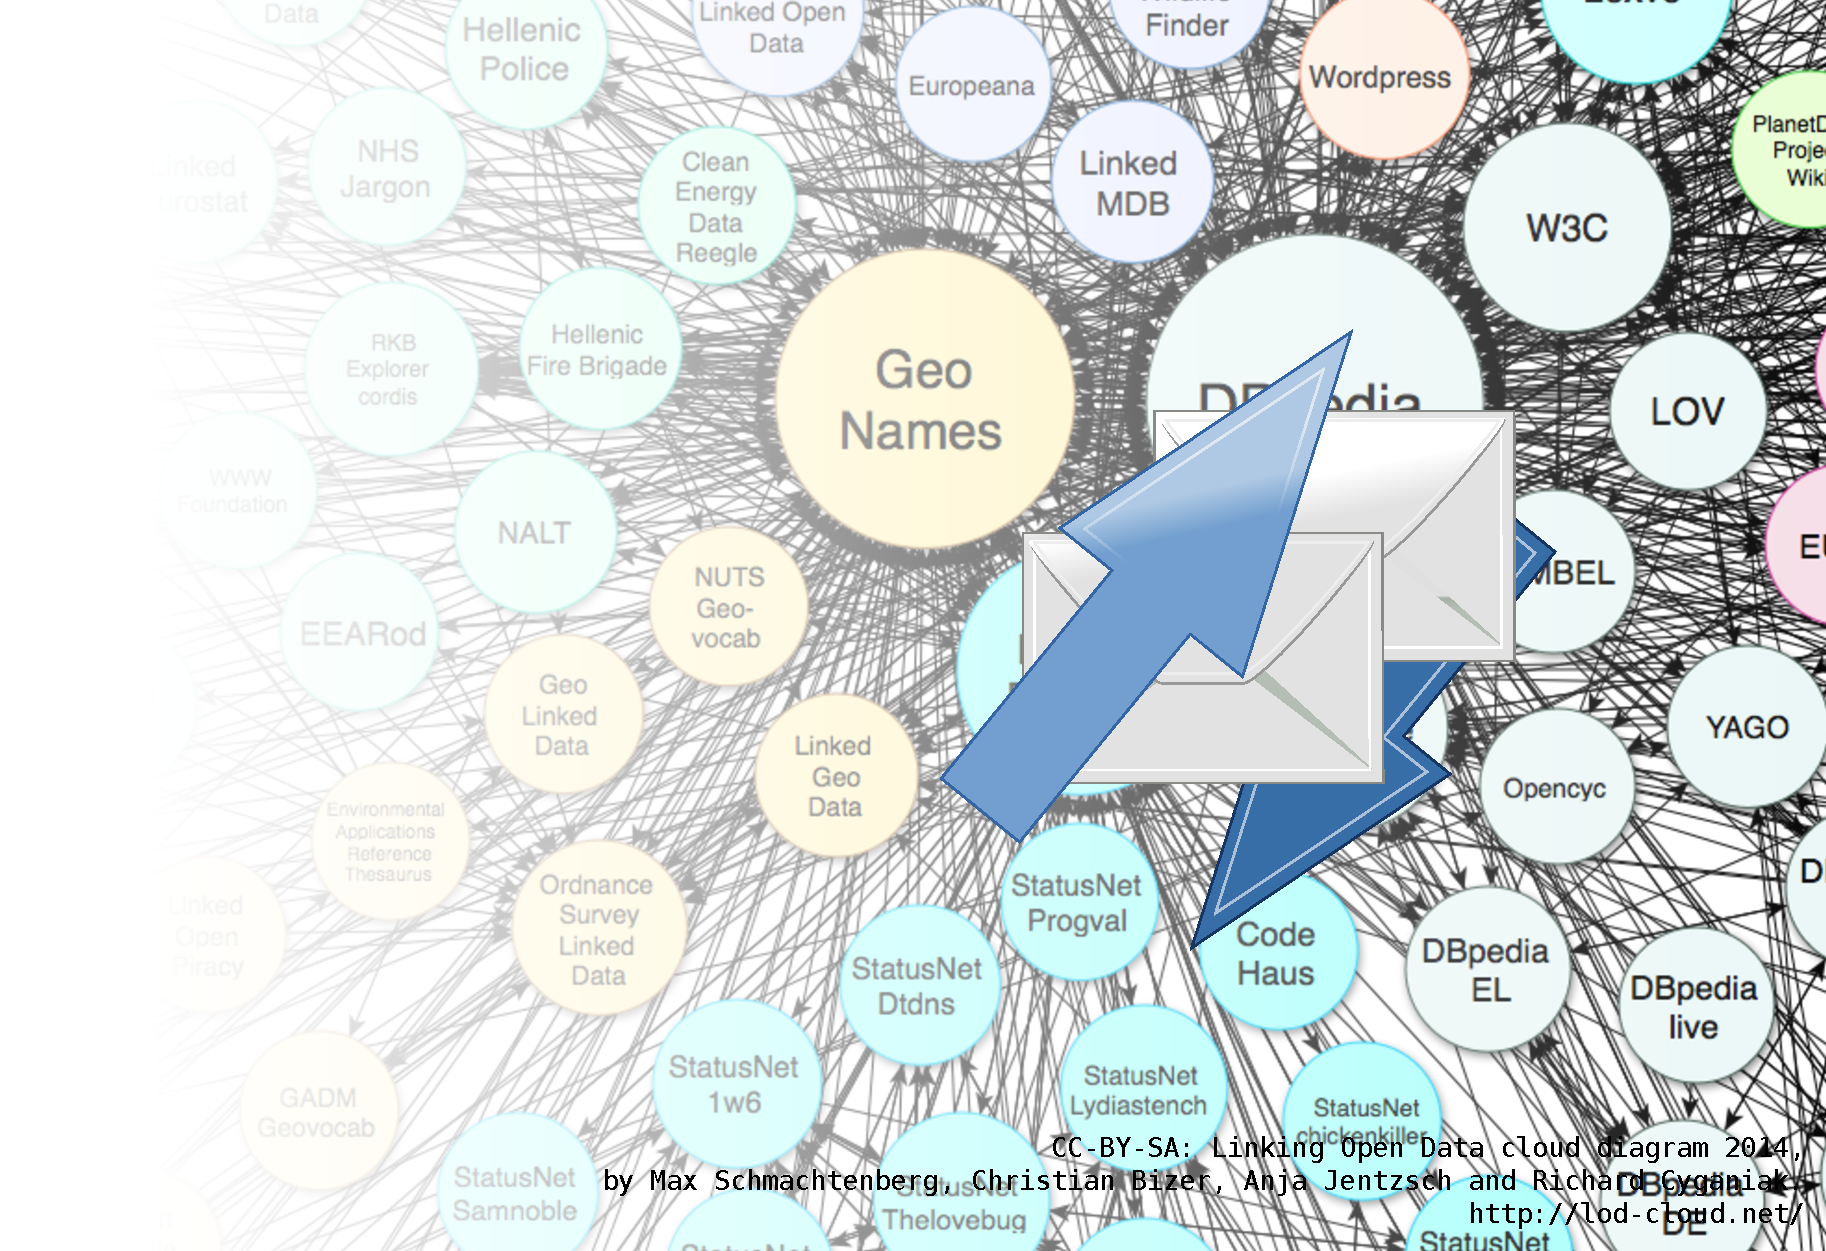
\includegraphics[width=.5\textwidth]{LOD-Cloud-2014_messages}};

  \begin{itemize}
  \item But currently there is no established way for \textbf{active communication}
  \item This is needed for …
  \begin{itemize}
  \item social interaction:\\messages, status update, friending; DSSN)
  \item subscription to updates of datasets; graph synchronization
  \item distributed collaboration on structured data
  \item enterprise use cases, such as distributed supply chain management
  \end{itemize}
  \end{itemize}

\end{frame}

\section{Linked Data Notifications (LDN)}
\subsection{W3C Working Draft}
\begin{frame}
  \frametitle{\insertsection: \insertsubsection}%
%   \framesubtitle{}%

  \begin{itemize}
    \item A Working Draft by the W3C Social Web Working Group
    \item Specialized use of Linked Data Platform (LDP)
    \item \url{https://www.w3.org/TR/2016/WD-ldn-20160824/} \cite{ldn}
  \end{itemize}
  
  \begin{quote}
   Linked Data Notifications is a protocol to facilitate exchanging messages between applications which serve as senders, receivers and/or consumers of RDF data.
  \end{quote} (Sarven Capadisli and Amy Guy: Linked Data Notifications)

\end{frame}


\subsection{Introduction}
\begin{frame}
  \frametitle{\insertsection: \insertsubsection}%
%   \framesubtitle{}%
\label{intro}

  \begin{itemize}
    \item Decoupling between applications and data storage
    \item A notification has its own URI which can be retrieved and reused
    \item The specification does not define the vocabulary of the notification contents
    \item Authentication and verification of notifications is encouraged
  \end{itemize}
\end{frame}


\subsection{Summary}
\begin{frame}
  \frametitle{\insertsection: \insertsubsection}%
%   \framesubtitle{}%
  
% \begin{minipage}{.5\textwidth}
  \begin{description}
    \item[Sender]
    \begin{itemize}
     \item Creates the notification body
     \item Sends the notification as \texttt{POST} to the Inbox URL
    \end{itemize}
 
    \item[Consumer]
    \begin{itemize}
     \item Retrieves the contents of the Inbox URL via \texttt{GET}
    \end{itemize}
    \item[Receiver]
    \begin{itemize}
     \item Responds to \texttt{GET} requests to the Inbox URL
     \item Accepts \texttt{POST} requests at the Inbox URL to create notifications
     \item Optionally enforces constraints on notifications
     %  sent to the Inbox. ->  sent to the Inbox and requested from the Inbox.
    \end{itemize}
  \end{description}
  
    \begin{figure}
     \begin{center}
     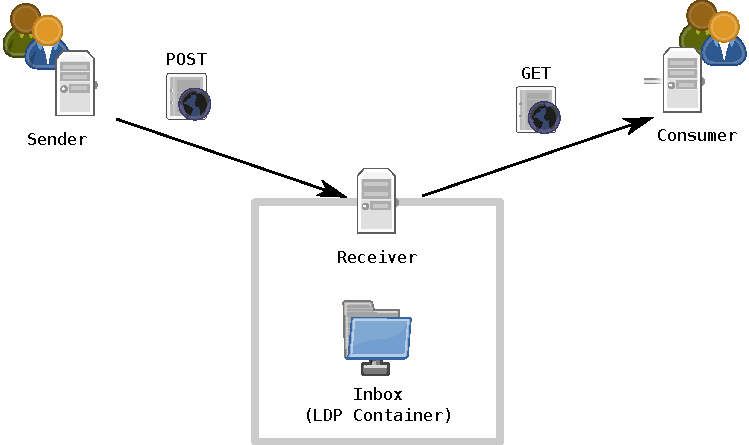
\includegraphics[width=.4\textwidth]{LingedDataNotifications/LDN-overview-1}
     \end{center}
    \end{figure}
  
\end{frame}


\subsection{Protocol – Discovery}
\begin{frame}
  \frametitle{\insertsection: \insertsubsection}%

  \begin{itemize}
   \item An Inbox can be discovered from any resource
   \item The starting point for discovery is the \textit{target}
   \item The \textit{sender} MUST make a request for a \qname{ldp:inbox} relation\\(\texttt{HEAD-Link} and \texttt{Linked Data})
  \end{itemize}

  
    \begin{figure}
     \begin{center}
     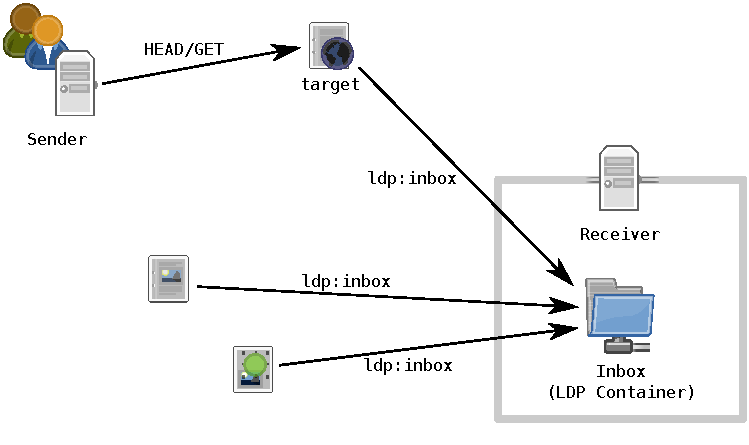
\includegraphics[width=.4\textwidth]{LingedDataNotifications/LDN-overview-discovery}
     \end{center}
    \end{figure}

\end{frame}


\subsection{Protocol – Sending and Receiving}
\begin{frame}
  \frametitle{\insertsection: \insertsubsection}%

  \begin{itemize}
   \item Senders MUST deliver notifications in a POST request to the Inbox URL
   \item The Receiver can delay processing of the notification: \texttt{202 Accepted}
   \item Or immediately answer with \texttt{201 Created} or the appropriate \texttt{4xx}
   \item Payload defaults to JSON-LD, but can be negotiated
   \item “The sender MUST NOT assume that the receiver can fetch or infer anything additional from the payload, and thus MUST include everything they want the receiver to know.”
  \end{itemize}

  
    \begin{figure}
     \begin{center}
     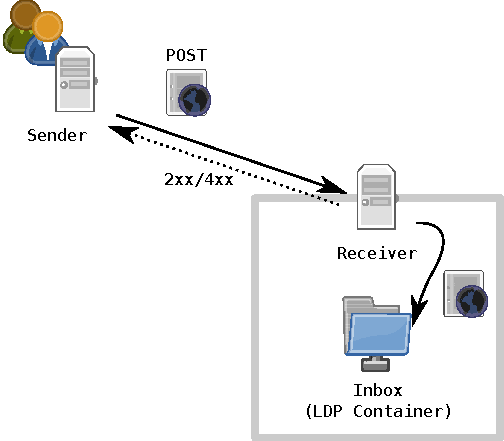
\includegraphics[width=.25\textwidth]{LingedDataNotifications/LDN-overview-sending}
     \end{center}
    \end{figure}

\end{frame}


\subsection{Protocol – Consuming}
\begin{frame}
  \frametitle{\insertsection: \insertsubsection}%

  \begin{itemize}
   \item The Receiver responds to \texttt{GET} requests on the Inbox URL
   \item Notifications must be discoverable through \qname{ldp:contains}
   \item Payload defaults to JSON-LD, but can be negotiated
  \end{itemize}

  
    \begin{figure}
     \begin{center}
     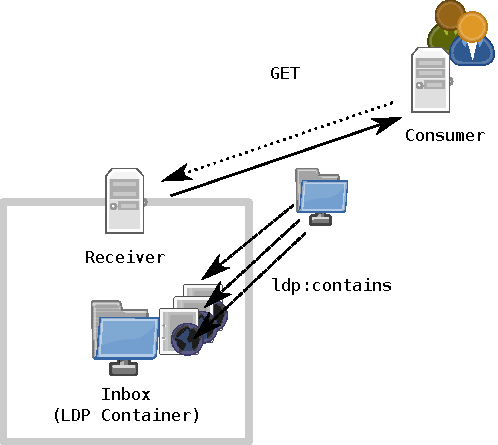
\includegraphics[width=.3\textwidth]{LingedDataNotifications/LDN-overview-consuming}
     \end{center}
    \end{figure}

\end{frame}


\subsection{Protocol – Security, Privacy and Content Considerations}
\begin{frame}
  \frametitle{\insertsection: \insertsubsection}%

  \begin{itemize}
   \item Inbox URLs can announce shape constraints
   \item consumers may want to take precautions when consuming notifications
   \item Receivers SHOULD ensure or verify the sender
   \begin{itemize}
    \item whitelist for write access
    \item require authentication
    \item retrieve a copy of the notification from the sender's domain to verify its origin
    \item checking a digital signature which accompanies the notification
   \end{itemize}

  \end{itemize}

\end{frame}


\subsection{Summary}
\begin{frame}
  \frametitle{\insertsection: \insertsubsection}%

    \begin{figure}
     \begin{center}
     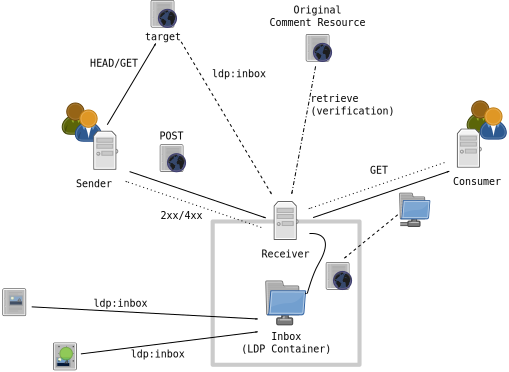
\includegraphics[width=.7\textwidth]{LingedDataNotifications/LDN-overview-all}
     \end{center}
    \end{figure}

\end{frame}

\section{Other Approaches}
\begin{frame}
  \frametitle{\insertsection}%

  \begin{itemize}
   \item The DSSN Stack \cite{tramp-s-2012--a} with PubSubHubbub and Semantic Pingback
   \item Applications in \emph{Structured Feedback}~\cite{arndt-2016-ldow-structured-feedback--} and \emph{Publish and Subscribe for RDF in Enterprise Value Networks}~\cite{frommhold-m-pubsub-2016}
  \end{itemize}

\end{frame}


\subsection{Publish and Subscribe for RDF in Enterprise Value Networks}
\begin{frame}
  \frametitle{\insertsection: \insertsubsection}%

    \begin{figure}
     \begin{center}
     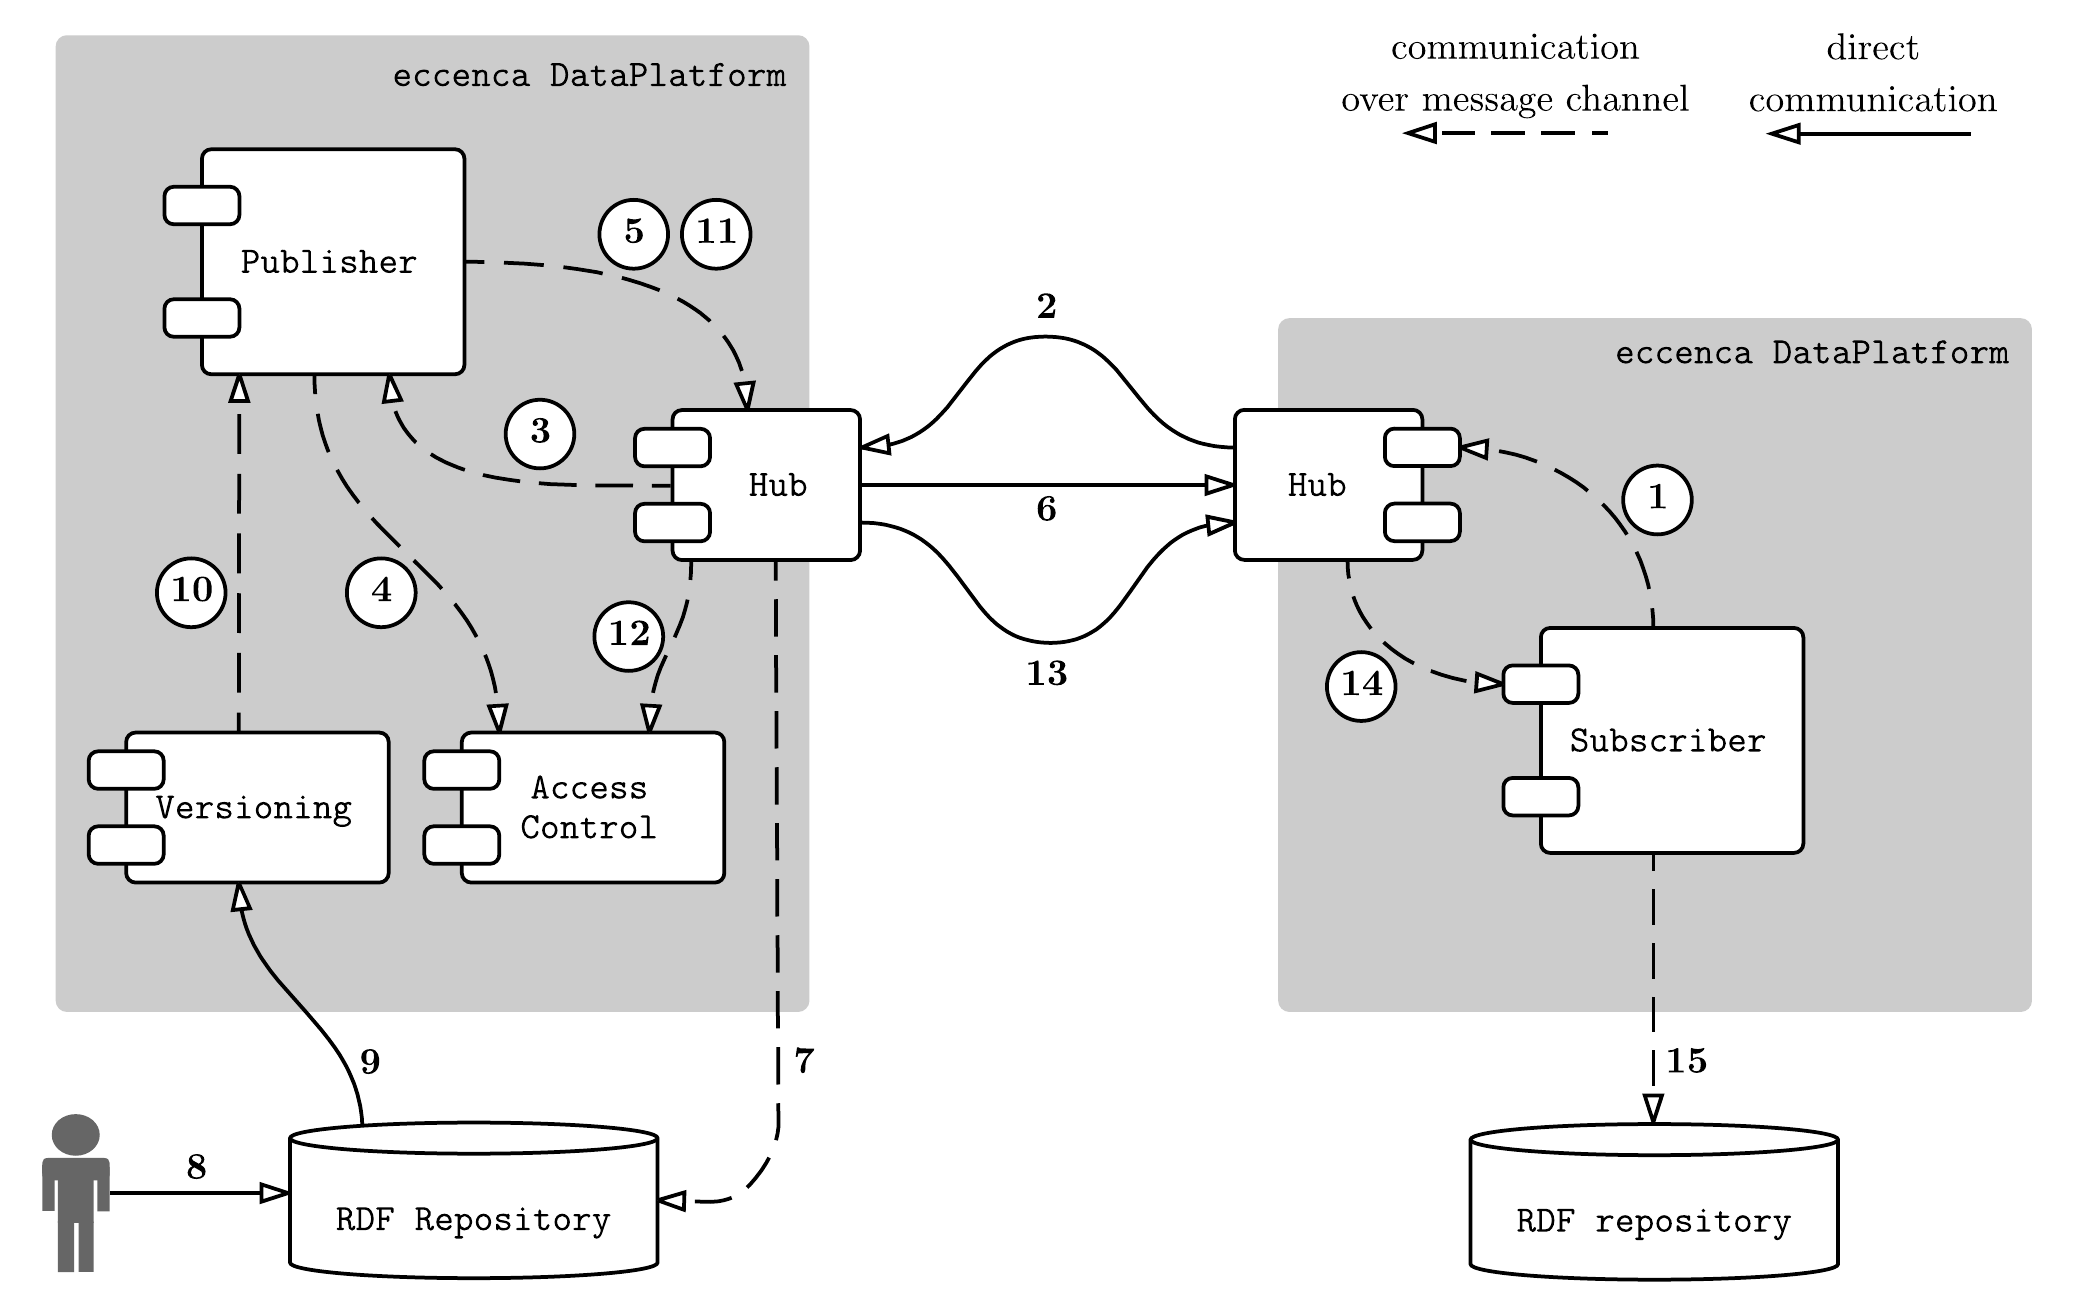
\includegraphics[width=.8\textwidth]{elds}
     \end{center}
    \end{figure}

\end{frame}

\subsection{Semantic Pingback and Structured Feedback}
\begin{frame}
  \frametitle{\insertsection: \insertsubsection}%

    \begin{figure}
     \begin{center}
     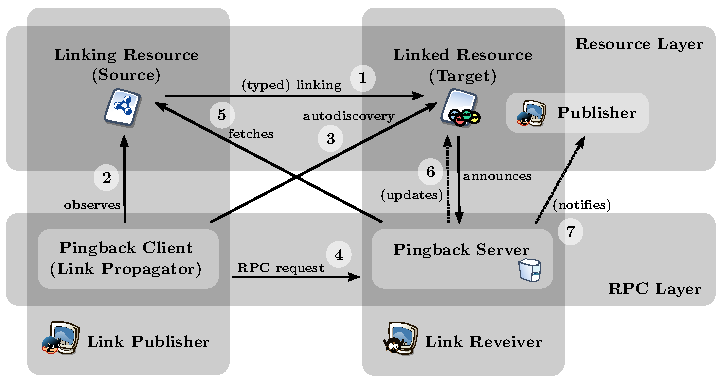
\includegraphics[width=.8\textwidth]{pingback}
     \end{center}
    \end{figure}

\end{frame}

\begin{frame}
  \frametitle{\insertsection: \insertsubsection}%

    \begin{figure}
     \begin{center}
     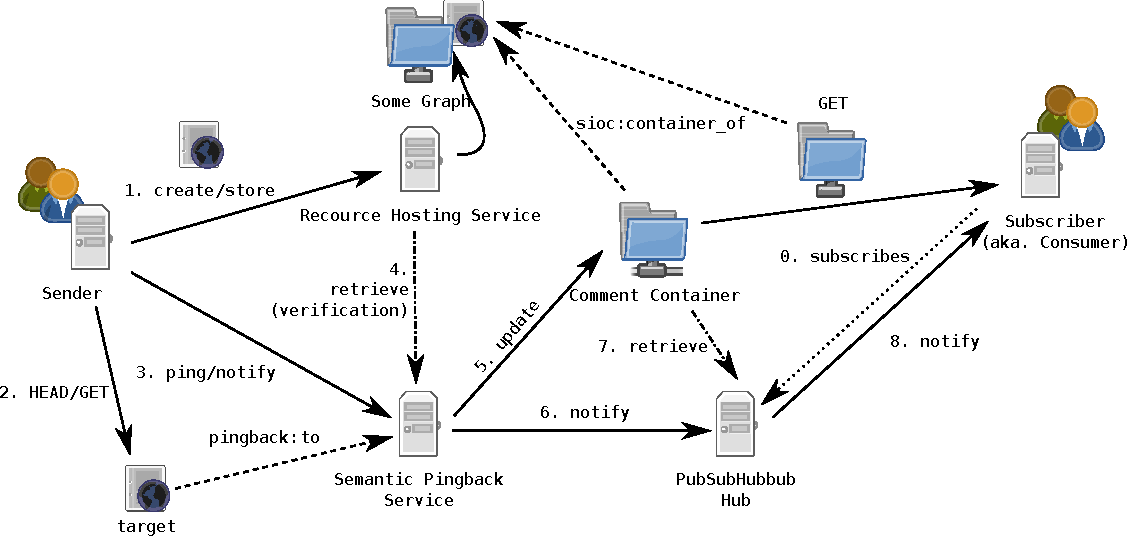
\includegraphics[width=.8\textwidth]{StructuredFeedback/SF-1}
     \end{center}
    \end{figure}

    \begin{itemize}
    \tiny
     \item In contrast to LDN the roll of the \emph{Receiver} is distributed among the \emph{Semantic Pingback Service} and the \emph{PubSubHubbub Hub}
     \item The roll of the \emph{Inbox} is done by the \emph{Comment Container}, while it doesn't necessarily be a LDP, but any Linked Data RDF
     \item The Actual notification resource stays at its origin and doesn't need to be copied and transfered for the protocol
    \end{itemize}
    
\end{frame}


\section{Discussion}
\begin{frame}
  \frametitle{\insertsection}%

  \begin{itemize}
   \item This Working Draft is a good starting point for active communication on Linked Data
   \item A W3C standard can help us to actually use RDF for communication and create meaningful communication
   \item Less polling, more pushing
  \end{itemize}

\end{frame}

\begin{frame}
  \frametitle{\insertsection}%

  
  \begin{itemize}
   \item Why using exactly JSON-LD as default and not any other RDF serialization?
   \item Why do all participants MUST support JSON-LD?
   \item Why should the payload replicate and contain the complete notification resource and the references information? Why not build links and reference it?
   \item “Decoupling between applications and data storage“ (\ref{intro}). Maybe also the tasks of the services and the different kinds of data storages can be decoupled.
   \item Why restrict the protocol to LDP and not also allow the resources to e.\,g. be managed by a SPARQL 1.1 endpoint?
  \end{itemize}

\end{frame}

\begin{frame}[allowframebreaks]
  \frametitle{References}
  \bibliographystyle{apalike}
  \bibliography{references}
\end{frame}

% \bibliographystyle{abbrv}

\end{document}
